\chapter{不定积分}
\section{不定积分的基本概念}
\defination[原函数]
如果在区间$I$上,可导函数$F(x)$的导函数为$f(x)$,即对任一$x\in I$都有
\begin{equation}
	F'(x)=f(x)\huo \d F(x)=f(x)\,\d x
\end{equation}
那么函数$F(x)$就称为$f(x)$(或$f(x)\,\d x$)在区间$I$上的一个\highlight{red}{原函数\index{YHS@{原函数}}}。\\
\kg 例如,$(\sin x)'=\cos x$,故$\sin x$是$\cos x$的一个原函数。
\\ 

\sj
\theorem[原函数存在定理]
如果函数$f(x)$在区间$I$上连续,那么在区间$I$上存在可导函数$F(x)$.使对任一$x\in I$都有
\begin{equation}
	F‘(x)=f(x)
\end{equation}
简单地说就是:\textbf{连续函数一定有原函数}(详见\ref{theorem:4}$\,$证明)
\warn[\kg 由于常数$C$的导数$(C)‘=0$,故一个函数的原函数有多个,可表示为$F(x)+C$($C$为常数)。]
\defination[不定积分]
在区间$I$上,函数$f(x)$的带有任意常数项的原函数称为$f(x)$(或$f(x)\,\d x$)在区间$I$上的不定积分,记作
\begin{equation}
	\int f(x)\,\d x
\end{equation}
其中记号$\di\int$称为积分号,$f(x)$称为被积函数,$f(x)\,\d x$称为被积表达式,$x$称为积分变量。

由此可知,如果$F(x)$是函数$f(x)$在区间$I$上的一个原函数,那么$F(x)+C$就是$f(x)$的\highlight{red}{\index{BDJF@不定积分}不定积分},即
\begin{equation}
	\int f(x)\,\d x=F(x)+C
\end{equation}
函数$f(x)$的原函数的图形称为$f(x)$的\highlight{red}{\index{JFQX@积分曲线}积分曲线}。
\section{不定积分的性质}
\vspace*{-1em}
\theorem[不定积分性质1]
设函数$f(x)$及$g(x)$的原函数存在,则
\begin{equation}
	\int [f(x)+g(x)]\,\d x=\int f(x)\,\d x+\int g(x)\,\d x
\end{equation}
\proof 设$f(x)$的原函数为$F(x)+C_1$,$g(x)$的原函数为$G(x)+C_2$,$f(x)+g(x)$的原函数为$F(x)+G(x)+C_3$,即
\sj
\begin{equation}
	\nonumber
	\int f(x)\,\d x=F(x)+C_1,\int g(x)\,\d x=G(x)+C_2,\int[f(x)+g(x)]\,\d x=F(x)+G(x)
+C_3\end{equation}
由于常数相加仍然是常数,即可令$C_3=C_1+C_2$,则上式成立。
\vspace*{0.5em}

\theorem[不定积分性质2]
设函数$f(x)$的原函数存在,则
\begin{equation}
	\int kf(x)\,\d x=k\int f(x)\,\d x
\end{equation}
\section{积分表}
\subsection{基本积分表}
\sj\sj
\begin{flalign*}
	\qquad & 1.\, \int k\,\d x=kx+C(k\text{为常数})   && 2.\, \int x^\mu\,\d x=\frac{x^{\mu+1}}{\mu+1}+C(\mu\neq-1)\vspace*{1em}&&\\[0.5em]
	\qquad & 3.\, \int \frac{\d x}{x}=\ln |x|+C   & &4.\, \int\frac{\d x}{1+x^2}=\arctan x+C\vspace{1em}&&\\[0.5em]
	\qquad & 5.\, \int\frac{\d x}{\sqrt{1-x^2}}=\arcsin x+C   && 6.\, \int \cos x \,\d x=\sin x+C\vspace{1em}&&\\[0.5em]
	\qquad & 7.\,\int\sin x \, \d x=-\cos x+C  && 8.\, \int \sec^2 x \,\d x=\tan x+C\vspace{1em}&&\\[0.5em]
	\qquad & 9.\,\int \csc^2 x \,\d x=-\cot x+C   &&10.\, \int \sec x\tan x \,\d x=\sec x+C\vspace{1em}&&\\[0.5em]
	\qquad & 11.\,\int \csc x\cot x \,\d x=-\csc x+C   & &12.\,\int \e^x \,\d x=\e^x+C\vspace{1em}&&\\[0.5em]
	\qquad & 13.\,\int a^x \,\d x=\frac{a^x}{\ln a}+C   
	&& 14.\, \int\text{sh} x \,\d x=\text{ch}x+C\vspace{1em}&&\\[0.5em]
	\qquad &15.\, \int \text{ch}x \,\d x=\text{sh}\hspace{0.2em} x+C   & &16.\,\int-\frac{\d x}{\sqrt{1-x^2}}=\arccos x+C\vspace{1em}&&\\[0.5em]
	\qquad &17.\, \int\frac{1}{\text{ch}^2x}\,\d x=\text{th}\hspace{0.2em} x+C   & &18.\, \int\frac{1}{\text{sh}^2x} \,\d x=-\frac{1}{\text{th }x}+C\vspace{1em}&&
\end{flalign*}
\vspace*{0.5em}

\subsection{扩展积分表}
注:下列常数$a>0$,部分内容涉及三角函数的变换(参阅章节 \ref{三角函数} )以及不定积分的运算法则(参阅章节 \ref{sec:1} )。
\newpage 

\noindent 19.\enspace $\di\int \tan x \,\d x=-\ln |\cos x|+C$
\vspace{1em}\\ \proof $\di\int \tan x \,\d x=\int \frac{\sin x}{\cos x} \,\d x=-\int\frac{1}{\cos x} \,\d (\cos x)=-\ln|\cos x|+C.$

\noindent 20.\enspace $\di\int \cot x \,\d x=\ln |\sin x|+C$\\[0.5em]
 \proof $\di\int \cot x \,\d x=\int \frac{\cos x}{\sin x} \,\d x=\int\frac{1}{\sin x} \,\d (\sin x)=\ln|\sin x|+C.$\\[1em]
21.\enspace $\di\int \csc x \,\d x=\int\frac{1}{\sin x} \,\d x=\frac{1}{2}\ln \bigg|\frac{1-\cos x}{1+\cos x}\bigg|+C=\ln\bigg |\tan \frac{x}{2}\bigg|+C=\ln|\csc x+\cot x|+C
$\\[1em]
\proof $\di\int \csc x \,\d x=\int \frac{1}{\sin x} \,\d x=\int\frac{\sin x}{\sin^2 x} \,\d x=-\frac{1}{1-\cos^2 x} \,\d (\cos x)=-\frac{1}{2}\int \bigg(\frac{1}{1-\cos x}+\frac{1}{1+\cos x}\bigg) \,\d(\cos x)$\\[0.5em]
\hspace*{9.5em}=$-\di\frac{1}{2}\ln \bigg|\di\frac{1+\cos x}{1-\cos x}\bigg|+C=\di\frac{1}{2}\ln \bigg|\di\frac{1-\cos x}{1+\cos x}\bigg|+C=\ln\bigg|\tan \frac{x}{2}\bigg|+C. $\\[1em]
22.\enspace $\di\int \sec x \,\d x=\int\frac{1}{\cos x} \,\d x=\frac{1}{2}\ln \bigg|\frac{1+\sin x}{1-\sin x}\bigg|+C=\ln|\sec x+\tan x|+C
$\\[1em]
\proof 证明与21相似,证明略.\\[1em]
23.\enspace $\di\int\frac{1}{a^2+x^2} \,\d x=\frac{1}{a}\arctan\frac{x}{a}+C$\\[1em]
\proof $\di\int\frac{1}{a^2+x^2} \,\d x=\frac{1}{a^2}\int\frac{1}{1+(\frac{x}{a})^2} \,\d x=\frac{1}{a}\int\frac{1}{1+(\frac{x}{a})^2}\,\d\bigg(\frac{x}{a}\bigg)=\frac{1}{a}\arctan\frac{x}{a}+C.$
\\[1em]
24.\enspace $\di\int\frac{1}{a^2-x^2} \,\d x=\frac{1}{2a}\ln \bigg|\frac{a+x}{a-x}\bigg|+C$\\[1em]
\proof $\di\int\frac{1}{a^2-x^2} \,\d x=\frac{1}{2a}\int\bigg(\frac{1}{a+x}+\frac{1}{a+x}\bigg) \,\d x=\frac{1}{2a}\ln \bigg|\frac{a+x}{a-x}\bigg|+C.$\\[1em]
25.\enspace$\di\int\frac{1}{\sqrt{a^2-x^2}} \,\d x=\arcsin \frac{x}{a}+C$\\[1em]
\proof $\di\int \frac{1}{\sqrt{a^2-x^2}} \,\d x=\frac{1}{a}\int\frac{1}{\sqrt{1-(\frac{x}{a})^2}}\d \bigg(\frac{x}{a}\bigg)=\arcsin \frac{x}{a}+C.$\\[1em]
26.\enspace $\di\frac{1}{\sqrt{x^2\pm a^2}} \,\d x=\ln \big| \, x+\sqrt{x^2\pm a^2}\,\big|+C$\\[1em]
\proof 由于正负号证法相似,故下面只证明正号情况。\\
令$x=a\tan t \, \bigg(\di-\frac{\pi}{2}<t<\frac{\pi}{2}\bigg)$,则
$$
\displaystyle \int \frac{1}{\sqrt{x^2+a^2}} \,\d x=\int\frac{a\sec^2 t}{\sqrt{a^2\sec^2t}} \,\d t=\int \frac{1}{\cos t} \,\d t=\frac{1}{2}\ln \bigg|\frac{1+\sin t}{1-\sin t}\bigg|+C=\ln |\sec t+\tan t|+
$$
如图 \ref{retri} 所示的直角三角形,可知当$\tan t=\di\frac{x}{a}$时,$\sec t=\di\frac{\sqrt{x^2+a^2}}{a}$,由上式得,\\[1em]
$\di\int\frac{1}{\sqrt{x^2+a^2}}\,\d x=\ln|\sec t+\tan t|+C=\ln\bigg|\frac{x}{a}+\frac{\sqrt{x^2+a^2}}{a}\bigg|+C=\ln\big|x+\sqrt{x^2+a^2}\big|+C'.$\\[1em]
\begin{figure}
	\centering
	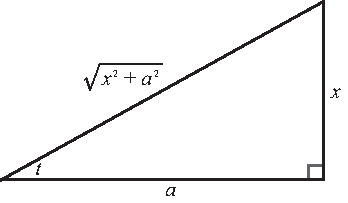
\includegraphics[width = 0.4\linewidth]{pic/C-3/retri}
	\vspace*{-1em}
	\caption{三角函数之间的关系}
	\label{retri}
\end{figure}

\noindent 27.\enspace $\di\int \sqrt{x^2\pm a^2} \,\d x=\frac{x}{2}\sqrt{x^2\pm a^2}+\frac{a^2}{2}\ln\big(\, x+\sqrt{x^2\pm a^2}\,\big)+C$\\[1em]
\proof 由于正负号证法相似,故下面只证明正号的情况.
\begin{align*}
\int \sqrt{x^2+a^2} \,\d x &=\int (x)'\sqrt{x^2+a^2} \,\d x=x\sqrt{x^2+a^2}-\int x(\sqrt{x^2+a^2})' \,\d x=x\sqrt{x^2+a^2}-\int\frac{x^2}{\sqrt{x^2+a^2}} \,\d x&\\[0.5em]
&=x\sqrt{x^2+a^2}-\int\frac{x^2+a^2-a^2}{\sqrt{x^2+a^2}} \,\d x=x\sqrt{x^2+a^2}-\int\sqrt{x^2+a^2} \,\d x+\int \frac{a^2}{\sqrt{x^2+a^2}} \,\d x&\\[0.5em]
&=x\sqrt{x^2+a^2}-\int \sqrt{x^2+a^2} \,\d x+a^2\int\frac{1}{\sqrt{x^2+a^2}} \,\d x&
\end{align*}
故$\di\int\sqrt{x^2+a^2} \,\d x=x\sqrt{x^2+a^2}-\int\sqrt{x^2+a^2} \,\d x+a^2\ln\big|\, x+\sqrt{x^2+a^2}\,\big|$,即
\begin{equation}
	\nonumber
	2\int\sqrt{x^2+a^2} \,\d x=x\sqrt{x^2+a^2}+a^2\ln\big|\, x+\sqrt{x^2+a^2}\,\big|.
\end{equation}
\begin{equation}
	\nonumber
	\int \sqrt{x^2+a^2} \,\d x=\frac{x}{2}\sqrt{x^2+a^2}+\frac{a^2}{2}\ln\left( \, x+\sqrt{x^2+a^2}\,\right)+C.
\end{equation}
\vspace*{0.5em}


\section{不定积分的运算法则}
\label{sec:1}
\subsection{第一类换元法}
\theorem[第一类换元法]
 设$f(x)$的原函数为$F(x)$,$u=u(x)$可导,则有换元公式
\begin{equation}
	\int f[u(x)]u'(x) \,\d x=\int f(u) \,\d u
\end{equation}
\myitem{\textbf{定理的应用}\\
	\kg 本质上是运用公式$u'(x) \,\d x=\d u$进行换元,使得$f(x)$变为$f(u)$后更容易求得积分。有些时候为了方便求出积分,在利用这个公式前需要进行对$f(x) \,\d x$进行构造变换成$f(u) \,\d u$的形式,下面给出几个例题具体说明。}
\clearpage
\vspace*{-3em}
\examples 求$\di\int 2\cos 2x \, \d x$.

\solvereason 观察式子,可以发现令$u=2x$,而易知$\d(2x)=2 \,\d x$.

\solve $\di\int 2\cos 2x \,\d x=\int \cos 2x \,\d(2x)=\int \cos u \,\d u=\sin u+C=\sin 2x+C.$\vspace*{-0.5em}
\warn[\kg 在普通的积分式中通常有一个隐含条件:$(x)'=1$,有时候这是构造的关键,就像本题应完整写为:
\begin{equation}
	\nonumber
	\int 2\cos 2x \,\d x=\int \cos 2x(2x)' \,\d x=\int \cos 2x \,\d(2x)=\int \cos u \,\d u=\sin u+C=\sin 2x+C.
	\end{equation}
但因为书写的简洁性与方便性,可以省略$(x)'=1$的步骤,$(x)'=1$的更多应用见第二类换元法。]

\examples 求$\di\int x\sqrt{1-x^2} \,\d x$

\solvereason 观察式子,注意到根式内含有二次项,根号外含有一次项,故联想$\d(x^2)=2x \,\d x.$

\solve $\di\int x\sqrt{1-x^2} \,\d x=\frac{1}{2}\int \sqrt{1-x^2} \,\d(x^2)=-\frac{1}{2}\cdot\frac{2}{3}(1-x^2)^{\frac{3}{2}}+C=-\frac{1}{3}(1-x^2)^{\frac{3}{2}}+C.$\vspace*{-0.5em}
\warn[\kg 在对变量换元的方法熟悉后,可以不写出换元的过程。]
\vspace*{0.1em}

\subsection{第二类换元法}
\vspace*{-1em}
\theorem[第二类换元法]  设$f(x)$的原函数为$F(x) , \,x=\varphi(t) \neq 0$是单调可导的函数.假设$f[\varphi (t)],\, \varphi'(t)$存在原函数,则有换元公式
\begin{equation}
	\di\int f(x) \,\d x=\int f[\varphi(t)] \,\d [\varphi(t)]=\int f[\varphi(t)]\varphi'^{(t)} \,\d t
\end{equation}
\myitem{\textbf{定理的应用}\\
\kg 本质上是将原变量$x$换成另外一个变量$t$使得原来不易求的积分式转换成另一个易求的积分式,即先找到这两个变量之间的函数关系$x=\varphi (t)$,再利用公式$\d x=\d[\varphi(t)]=\varphi'(t) \,\d t$进行微分变量的转换,这里要强调的是最后的结果仍然要用原来的变量$x$来表示,即将变量$t$再转化为原变量$x$,只需将$t=\varphi^{-1}(x)$代入即可。下面给出几个例题具体说明。}
\vspace{-0.5em}

\noindent \examples 求$\di\int \sqrt{a^2-x^2} \,\d x.(a>0)$
\vspace*{-0.5em}

\solvereason 观察式子,由基本公式的补充公式(见附章)联想到$\sin^2 x+\cos^2 x=1$来化去根式。\\[1em]
\solve 设$\di x=a\sin t,-\frac{\pi}{2}<t<\frac{\pi}{2}$,则$\sqrt{a^2-x^2}=\sqrt{a^2-a^2\sin^2 t}=a\cos t,\d x=\d(a\sin t )=a\cos t \,\d t$,则
\sj
\begin{align*}
	\int \sqrt{a^2-x^2}\,\d t&=\int a\cos t\cdot a\cos t \,\d t=a^2\int \cos^2 t \,\d t=a^2\int \frac{1+\cos 2t}{2} \,\d t=\frac{t^2}{2}\bigg(\int 1 \,\d t+\int \cos 2t \,\d t\bigg)&\\[0.3em]
	&=\frac{a^2}{2}\bigg(t+\frac{1}{2}\sin 2t\bigg)+C
\end{align*}
由于$x=a\sin t$,故$t=\arcsin\di\frac{x}{a}$,则$\di\cos t=\sqrt{1-\sin^2 t}=\sqrt{1-\bigg(\frac{x}{a}\bigg)^2}=\frac{\sqrt{a^2-x^2}}{a}$,即
\begin{align*}
	\int \sqrt{a^2-x^2}&=\frac{a^2}{2}\bigg(t+\frac{1}{2}\sin 2t\bigg)+C=\frac{a^2}{2}t+\frac{a^2}{2}\sin t\cos t+C=\frac{a^2}{2}\arcsin \frac{x}{a}+\frac{a^2}{2}\cdot\frac{x}{a}\cdot\frac{\sqrt{a^2-x^2}}{a}+C&\\[0.5em]
	&=\frac{a^2}{2}\arcsin\frac{x}{a}+\frac{1}{2}x\sqrt{a^2-x^2}+C.
\end{align*}
\sj\sj
\warn[\kg 对于求含有根号且根号内某两个数具备平方差(和)的关系时的积分,我们通常会进行三角换元从而去根号,然后再运用三角函数的公式进行化简和变形,这就要求我们要熟记并能灵活运用附章中关于三角函数的所有公式。下面给出一个新颖的三角函数公式进行换元的例子。]
\examples 求$\di\int \cot^4 x \,\d x.$

\solvereason 观察式子,由基本公式的补充公式(见附章)联想到$\csc^2 x-\cot^2 x=1$来进行降幂。

\solve 
$	\di\int \cot^4 x \,\d x=\int \cot ^2 x(\csc^2 x-1) \,\d x=\int \cot^2 x\csc^2 x \,\d x-\int \cot^2 x \,\d x$\\
\hspace*{9.8em}$\di	=-\int\cot^x \,\d(\cot x)-\int(\csc^2-1) \,\d x=-\frac{1}{3}\cot^3 x+\cot x+x+C.$
\vspace*{0.5em}

\subsection{分部积分法}
	设函数$u=u(x)$及$v=v(x)$具有连续导数,则两个函数乘积的导数公式为
	\begin{equation}
		(uv)'=u'v+uv'
	\end{equation} 
移项得
\begin{equation}
	uv'=(uv)'-u'v
	\end{equation}
对这个等式两边求不定积分,得
\begin{equation}
	\int uv' \,\d x=uv-\int u'v \,\d x
\end{equation}
方便期间,我们可以利用$u'\d x=\d u,v'\d x=\d v$进行转换,写成下列形式
\begin{equation}
	\int u \,\d v=uv-\int v \,\d u
\end{equation}
这个公式称为\highlight{red}{\index{FBJFGS@分部积分公式}分部积分公式}.\\
\myitem{\textbf{定理的应用}\\
\kg 如果求$\di\int u \,\d v$有困难,而求$\di\int v \,\d u$比较容易时,这个公式就给了我们一个很便捷的思路。}\vspace{1em}
\examples 求$\di\int x\cos x \,\d x.$\\
\solve $\di\int x\cos x \,\d x=\int x \,\d \sin x=x\sin x-\int \sin x \,\d x=x\sin x+\cos x+C $




